\documentclass{beamer}


% Vary the color applet  (try out your own if you like)
%\colorlet{structure}{red!65!black}

%\beamertemplateshadingbackground{yellow!100}{white}

\usepackage{beamerthemesplit}
\usepackage{graphics}
\usepackage{graphicx}
\usepackage{hyperref}



\title[dMRI]{Sparse Reconstruction of Diffusion MRI signals}
\author[]{}
%
\institute[]{
  \begin{tabular}[h]{cc}
      \large{Cory Ahrens}                         & \large{Fernando P\'{e}rez}  \\
      \large{Jennifer Nealy}                      & \large{St\'{e}fan van der Walt} \vspace{0.2em}\\
      Dept of Applied Mathematics and Statistics  &  Helen-Wills Neuroscience Institute \\
      Colorado School of Mines                    &  University of California, Berkeley \\
      Golden, CO 80401                            &  Berkeley, CA 94720
  \end{tabular}      
}
\date[April XXX 2013]{ISBI-2013}
\subject{Computational Sciences}

\pgfdeclaremask{csm}{csm_logo}
\pgfdeclareimage[mask=csm,width=3cm]{csm-logo}{csm_logo}

\logo{\vbox{\vskip0.1cm\hbox{\pgfuseimage{csm-logo}}}}

\begin{document}

  \frame
  {
    \titlepage
  }
%==========================================================%
%==========================================================%
  \section{Outline}
%==========================================================%
  \frame
  {
    \frametitle{Outline}
    \tableofcontents
    %\begin{itemize}
      %\item<1-> Normal LaTeX class.
      %\item<2-> Easy overlays.
      %\item<3-> No external programs needed.      
    %\end{itemize}
  }

%==========================================================%
%==========================================================%
%==========================================================%
  \section{Diffusion MRI}
%==========================================================%
  \frame
  {
    \frametitle{Background} 
    Diffusion MRI can be used to determine ``connectivity'' in the brain \emph{in vivo}. 
  \begin{center}
    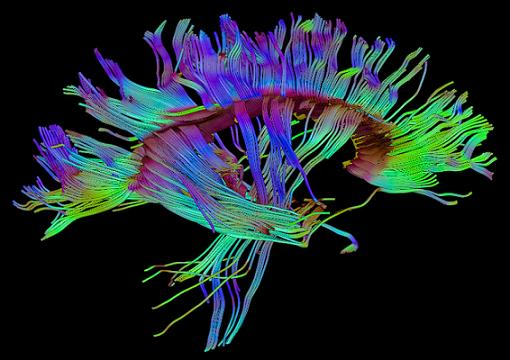
\includegraphics[width = 2.25in]{MRI-DTIBrain-9223.jpg}
  \end{center}

  }%==========================================================%
  \frame
  {
    \frametitle{Basic formulation} 
    Diffusion MRI measurements are taken in the Fourier domain:
    \begin{equation}
      E\left(\mathbf{k}\right) = \frac{s\left(\mathbf{k}\right)}{s_0} = \int_{\mathbb{R}^3} p\left(\mathbf{r}\right)e^{i \mathbf{k}\cdot\mathbf{r}}d^3\mathbf{r}
    \end{equation}
    \begin{itemize}
      \item{$\mathbf{k} \sim $ applied magnetic field gradients}
      \item{Reconstruction of $p\left(\mathbf{r}\right)$ requires many samples in $\mathbf{k}$-space}
      \item{Each sample is a measurement: more measurements $\rightarrow$ longer clinical times $\rightarrow$ unhappy patients}
      \item{Primarily need directional information from $p\left(\mathbf{r}\right)$, i.e., want to recover $p\left(\mathbf{r}\right)$ with $\mathbf{r}\in\mathbb{S}^2$}
    \end{itemize}
  }
%==========================================================%
  \frame
  {
  \frametitle{Reconstruction of PDF} 
    \begin{itemize}
      \item{Initial reconstruction algorithms for $p\left(\boldsymbol{\Omega}\right)$ based on Gaussian ansatz -- recovers diffusion tensor, sampling on $\mathbf{k}$ shell}
      \item{Diffusion tensor imaging (DTI) is limited in angular resolution and can resolve only one primary direction per voxel}
      \item{Now people use High-Angular-Resolution-Diffusion-Imaging (HARDI) -- there is not one accepted formulation of HARDI}
      \item{Main idea in HARDI -- integrate out radial component of FT to get equation for ``orientation distribution function'' -- a PDF on the sphere, $\phi\left(\boldsymbol{\Omega}\right)$}
      \item{ODF should be peaked in dominant direction(s) of fiber(s)}
      \item{Spherical harmonics are not so good for ``localized'' features...try new representation instead}
    \end{itemize}
  }
%==========================================================%
  \frame
  {
    \frametitle{Formulation} 
    One formulation of HARDI is
    \begin{equation}
      \phi\left(\boldsymbol{\Omega}\right) = -\frac{1}{4\pi^2}\mathcal{G}\left[\Delta E\left(\boldsymbol{\Omega}\right) \right],  
    \end{equation}
    where $\phi\left(\boldsymbol{\Omega}\right)$ is the ODF, $E\left(\boldsymbol{\Omega}\right)$ is the measured signal, $\Delta$ is the Laplacian restricted to the sphere and $\mathcal{G}$ is the Funk-Radon transform
    \begin{equation}
      \mathcal{G}\phi\left(\boldsymbol{\Omega}\right) = \int_{\mathbb{S}^2} \delta\left(\boldsymbol{\Omega}\cdot\boldsymbol{\Omega}'\right)f\left(\boldsymbol{\Omega}'\right)d^2\boldsymbol{\Omega}'
    \end{equation}
 
  }
%==========================================================%
  \frame
  {
    \frametitle{Formulation} 
    If $\phi$ is to have the representation 
    \begin{equation}
      \phi\left(\boldsymbol{\Omega}\right) = \sum_{i=1}^M \phi_i K_e\left(\boldsymbol{\Omega}\cdot\boldsymbol{\Omega}_i\right),  
    \end{equation}
    (with $\boldsymbol{\Omega}_i$, $i=1,2,...,M$ quadrature points) then we need to represent the measured signal $E$ as linear combinations of
    \begin{equation}
      H\left(\mu\right)\equiv-\sum_{n=1}^{\left\lfloor N/2\right\rfloor }\frac{2\left(2n\right)+1}{8\pi^{2}P_{2n}\left(0\right)\left(2n\right)\left(2n+1\right)}P_{2n}\left(\mu\right),
    \end{equation}
    where $P_n\left(\mu\right)$ is the $n^{th}$ degree Legendre polynomial.
  }
%==========================================================%
  \frame
  {
    \frametitle{Formulation} 
    That is, we have the following linear system to solve:
    \begin{equation}
      E\left(\boldsymbol{\Omega}_{j}\right) \thickapprox\sum_{i=1}^{M}\phi_{i}\, H\left(\boldsymbol{\Omega}_{j}\cdot\boldsymbol{\Omega}_{i}\right),\: j=1,2,3,\cdots M',
    \end{equation}
    where $E\left(\boldsymbol{\Omega}_{j}\right)$ are measured data and we want to determine the $\phi_i$. We then get $\phi\left(\boldsymbol{\Omega}\right)$ by \emph{analytically} applying the Laplacian and Funk-Radon transform. 

    We consider $M' < M$ and solve an $l_1$-penalized least-squares problem:
    \begin{equation}
      \mathrm{min} \lVert E\left(\boldsymbol{\Omega}_{j}\right) - \sum_{i=1}^{M}\phi_{i}\, H\left(\boldsymbol{\Omega}_{j}\cdot\boldsymbol{\Omega}_{i}\right)\rVert_{2} + \lambda \lVert\boldsymbol{\phi}\rVert_{1}
    \end{equation}
  }
%==========================================================%
  \frame
  {
  \frametitle{Preliminary results}
  A ``signal'' function $H$.
  \vspace{-0.1in}
  \begin{center}
    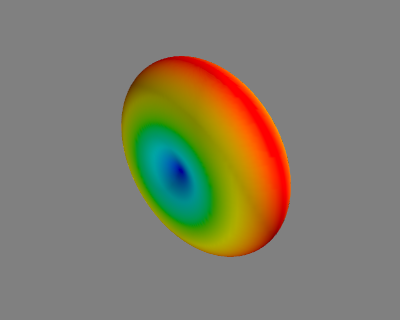
\includegraphics[width = 2.25in]{snapshot.png}
  \end{center}
  }

%==========================================================%
  \frame
  {
  \frametitle{Preliminary results}
  A single fiber reconstruction:
  \vspace{-0.1in}
  \begin{center}
    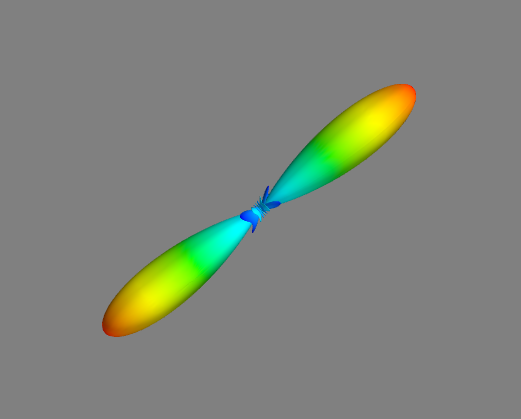
\includegraphics[width = 2.25in]{odf-1.png}
  \end{center}
  }

%==========================================================%
  \frame
  {
  \frametitle{Preliminary results}
  A two fiber ($90$ degree crossing) reconstruction:
  \vspace{-0.1in}
  \begin{center}
    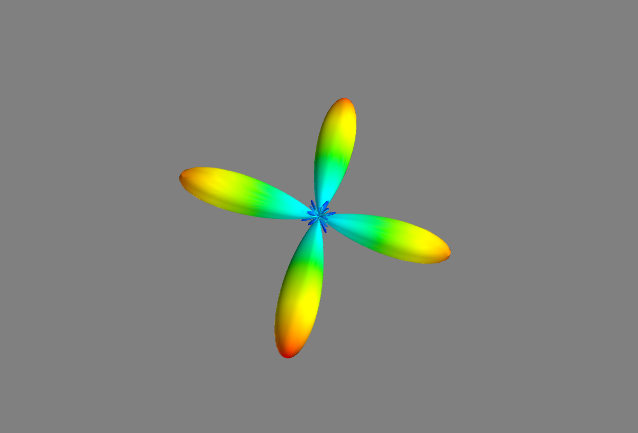
\includegraphics[width = 2.25in]{odf-2-90.png}
  \end{center}
  }
%==========================================================%
  \frame
  {
  \frametitle{Preliminary results}
  A two fiber ($45$ degree crossing) reconstruction:
  \vspace{-0.1in}
  \begin{center}
    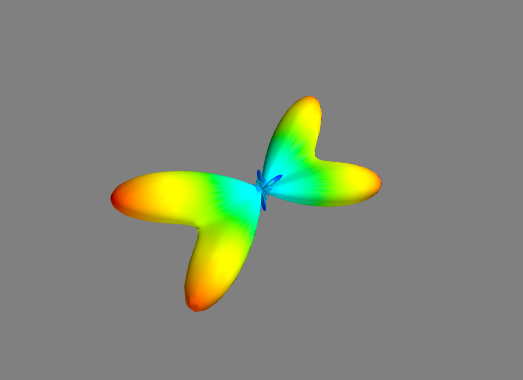
\includegraphics[width = 2.25in]{odf-2-45.png}
  \end{center}
  }
%==========================================================%


\end{document}
